% \documentclass[a4paper, conference, compsoc]{IEEEtran}
\documentclass[12pt,a4paper]{article}
% \documentclass[%
%     pdftex,
%     oneside,			% Einseitiger Druck.
%     12pt,				% Schriftgroesse
%     parskip=half,		% Halbe Zeile Abstand zwischen Absätzen.
% %	topmargin = 10pt,	% Abstand Seitenrand (Std:1in) zu Kopfzeile [laut log: unused]
%     headheight = 12pt,	% Höhe der Kopfzeile
% %	headsep = 30pt,	% Abstand zwischen Kopfzeile und Text Body  [laut log: unused]
%     headsepline,		% Linie nach Kopfzeile.
%     footsepline,		% Linie vor Fusszeile.
%     footheight = 16pt,	% Höhe der Fusszeile
%     abstracton,		% Abstract Überschriften
%     DIV=calc,		% Satzspiegel berechnen
%     BCOR=8mm,		% Bindekorrektur links: 8mm
%     headinclude=false,	% Kopfzeile nicht in den Satzspiegel einbeziehen
%     footinclude=false,	% Fußzeile nicht in den Satzspiegel einbeziehen
%     listof=totoc,		% Abbildungs-/ Tabellenverzeichnis im Inhaltsverzeichnis darstellen
%     toc=bibliography,	% Literaturverzeichnis im Inhaltsverzeichnis darstellen
% ]{scrreprt}	% Koma-Script report-Klasse, fuer laengere Bachelorarbeiten alternativ auch: scrbook


% Basic packages
\usepackage[T1]{fontenc}
\usepackage[utf8]{inputenc}
\usepackage[scaled]{beramono}
\usepackage[english,ngerman]{babel,varioref}
\usepackage{xcolor}
\usepackage{amsmath}

% Tables
\usepackage{booktabs}
\usepackage{multirow}
\usepackage{longtable}
% Graphics and Includes
\usepackage[pdftex]{graphicx}
\graphicspath{{assets/img/}}
\DeclareGraphicsExtensions{.pdf,.jpeg,.png,.jpg}
\usepackage{tikz}
\usetikzlibrary{arrows.meta,bending,automata,shapes}
\usepackage[underline=true,rounded corners=false]{pgf-umlsd}

% Reduce distance before caption
\usepackage[skip=5pt]{caption}
% Bibliography
\usepackage[backend=biber, isbn=false, doi=false, style=ieee]{biblatex}
\addbibresource{bibliography.bib}
\AtBeginBibliography{\raggedright}
%\nocite{*}

% Gossar z.a. für acronyme
% \usepackage[acronym]{glossaries}
% \makeglossaries
\usepackage[printonlyused]{acronym} % falls gewünscht kann die Option footnote eingefügt werden, dann wird die Erklärung nicht inline sondern in einer Fußnote dargestellt

% \section*{Abkürzungsverzeichnis}
\begin{acronym}[AAAAAA]
    \acro{sac}[SAC]{SAP Analytics Cloud}
    \acro{ux}[UX]{User Experience} 
    \acro{dod}[DoD]{Definition of Done}
    \acro{2d}[2D]{Zwei Dimensional}
    \acro{ui}[UI]{User Interface}
    \acro{arc}[ARC]{Area Release Check}
\end{acronym}
% Colors
\definecolor{ListingBackground}{HTML}{E6E6E6}
\definecolor{LinkColor}{HTML}{000000}


% Font
\usepackage[onehalfspacing]{setspace}
\usepackage{lmodern}
\usepackage[official]{eurosym}
\usepackage{enumitem}
\usepackage[locale=DE]{siunitx} % SI Units für Währungen
\DeclareSIUnit{\EUR}{\text{\euro}} % Beispielverwendung: \SI{10.10}{\EUR}

\usepackage[autostyle=true,german=quotes]{csquotes}
\usepackage{url}
\newcommand{\code}[1]{\texttt{#1}}

% Additional Setup
\usepackage[unicode=true,hypertexnames=false,colorlinks=true,linkcolor=LinkColor,citecolor=LinkColor,urlcolor=LinkColor,pdftex]{hyperref}

% Trennung von URLs im Literaturverzeichnis (große Werte [> 10000] verhindern die Trennung)
\defcounter{biburlnumpenalty}{10} % Strafe für Trennung in URL nach Zahl
\defcounter{biburlucpenalty}{500}  % Strafe für Trennung in URL nach Großbuchstaben
\defcounter{biburllcpenalty}{500}  % Strafe für Trennung in URL nach Kleinbuchstaben
\interfootnotelinepenalty=10000 % prevent all footnotes from breaking over a page.

% Configs
\setcounter{tocdepth}{1} % Limit table of contents to subsection
\sisetup{detect-weight=true, detect-family=true} % SI Units shall detect font weight and family
\setlist[description]{style=nextline} % Break definitions of terms to a new line (used by \begin{description} \item[foo] bar \end{description})
\renewcommand*{\bibfont}{\small}

%Hurenkinder und Schusterjungen vermeiden
\clubpenalty = 10000
\widowpenalty = 10000
\displaywidowpenalty = 10000

% Quellcode
\usepackage{listings}
\usepackage{float}
\usepackage{textcomp}
\lstset{
    inputpath=assets/listings,
    language=Java,			% Standardsprache des Quellcodes
    numbers=left,			% Zeilennummern links
    stepnumber=1,			% Jede Zeile nummerieren.
    numbersep=5pt,			% 5pt Abstand zum Quellcode
    numberstyle=\tiny,		% Zeichengrösse 'tiny' für die Nummern.
    breaklines=true,		% Zeilen umbrechen wenn notwendig.
    breakautoindent=true,	% Nach dem Zeilenumbruch Zeile einrücken.
    postbreak=\space,		% Bei Leerzeichen umbrechen.
    tabsize=2,				% Tabulatorgrösse 2
    basicstyle=\ttfamily\footnotesize, % Nichtproportionale Schrift, klein für den Quellcode
    showspaces=false,		% Leerzeichen nicht anzeigen.
    showstringspaces=false,	% Leerzeichen auch in Strings ('') nicht anzeigen.
    extendedchars=true,		% Alle Zeichen vom Latin1 Zeichensatz anzeigen.
    captionpos=b,			% sets the caption-position to bottom
    backgroundcolor=\color{ListingBackground}, % Hintergrundfarbe des Quellcodes setzen.
    xleftmargin=0pt,		% Rand links
    xrightmargin=0pt,		% Rand rechts
    frame=single,			% Rahmen an
    frameround=ffff,
    rulecolor=\color{darkgray},	% Rahmenfarbe
    fillcolor=\color{ListingBackground},
    keywordstyle=\color[rgb]{0.133,0.133,0.6},
    commentstyle=\color[rgb]{0.133,0.545,0.133},
    stringstyle=\color[rgb]{0.627,0.126,0.941},
    float,
    upquote=true
}


\colorlet{punct}{red!60!black}
\definecolor{delim}{RGB}{20,105,176}
\colorlet{numb}{magenta!60!black}

\lstdefinelanguage{json}{
    string=[s]{"}{"},
    stringstyle=\color{numb},
    literate=
     *{0}{{{\color{numb}0}}}{1}
      {1}{{{\color{numb}1}}}{1}
      {2}{{{\color{numb}2}}}{1}
      {3}{{{\color{numb}3}}}{1}
      {4}{{{\color{numb}4}}}{1}
      {5}{{{\color{numb}5}}}{1}
      {6}{{{\color{numb}6}}}{1}
      {7}{{{\color{numb}7}}}{1}
      {8}{{{\color{numb}8}}}{1}
      {9}{{{\color{numb}9}}}{1}
      {:}{{{\color{punct}{:}}}}{1}
      {,}{{{\color{punct}{,}}}}{1}
      {\{}{{{\color{delim}{\{}}}}{1}
      {\}}{{{\color{delim}{\}}}}}{1}
      {[}{{{\color{delim}{[}}}}{1}
      {]}{{{\color{delim}{]}}}}{1}
}

\lstdefinelanguage{yaml}{
  identifierstyle=\color{delim},
  sensitive=false,
  comment=[l]{\#},
  commentstyle=\color{purple}\ttfamily,
  stringstyle=\color{numb},
  morestring=[b]',
  morestring=[b]"
}

\lstloadlanguages{Python,Java,bash}
% Useful tools
\usepackage{blindtext}
\usepackage{lipsum}
\usepackage[section]{placeins} % Prevent figures and tables to float to new section
\usepackage[obeyFinal,backgroundcolor=yellow,linecolor=black]{todonotes}


%Angaben zur Arbeit
\def\myTitel{Kriterien für die Ideenbewertung}
\def\myArbeit{Seminararbeit}
\def\myFach{Forschungsmethoden und Innovation}
\def\myDatum{\today}
\def\myBetreuer{Prof. Dr. Florian Simons}
\def\myGutachter{Strenger Gutachter}
\def\myBearbeitungszeit{Lange}
\def\myAbgabeort{Heilbronn}

%Angaben zur Person
\def\myAutor{Lea Poletin}
\def\myDegree{Master Informatik}
\def\myInstitution{DHBW CAS, Bildungscampus 13, 74076 Heilbronn}
\def\myMatrikelnr{8514262}
\def\myKurs{TMINF17}
\def\myFirma{SAP SE}
\def\myFirmenort{Walldorf}
%\section*{Abkürzungsverzeichnis}
\begin{acronym}[AAAAAA]
    \acro{sac}[SAC]{SAP Analytics Cloud}
    \acro{ux}[UX]{User Experience} 
    \acro{dod}[DoD]{Definition of Done}
    \acro{2d}[2D]{Zwei Dimensional}
    \acro{ui}[UI]{User Interface}
    \acro{arc}[ARC]{Area Release Check}
\end{acronym}
\begin{document}


\title{\myTitel}
\author{\myAutor~(\myMatrikelnr)\\
    \small{\myFach}\\
    \small{\myDegree}\\
    \small{\myInstitution}
}
\date{\myDatum}

\begin{titlepage}
	\begin{longtable}{p{8.2cm} p{5.4cm}}
		% Firmenlogo
		&
		
\includegraphics[width=5.4cm]{casLogo}
	\end{longtable}
	\addtocounter{table}{-1}
    {\let\newpage\relax\maketitle}
    \thispagestyle{empty}
    % \vfill
    \begin{abstract}
   Diese Seminararbeit widmet sich dem Thema \textit{Kriterien für die Ideenbewertung}. Es werden Konzepte und Verfahren 
   vorgestellt, die beschreiben, wie Kriterien entwickelt, strukturiert und angewendet werden können. Anhand von zwei 
   praktischen Beispielen, wird die Anwendung von Kriterien zur Ideenbewertung beschrieben. 
\end{abstract}
\end{titlepage}
% \begin{titlepage}
	\begin{longtable}{p{8.2cm} p{5.4cm}}
		% Firmenlogo
		&
		
\includegraphics[width=5.4cm]{casLogo}
	\end{longtable}
	\addtocounter{table}{-1}
	\enlargethispage{20mm}
	\begin{center}
		\vspace*{12mm}	{\LARGE\textbf \myTitel }\\
		\vspace*{12mm}	{\large\textbf \myArbeit}\\
		% \vspace*{12mm}	\langdeckblattabschlusshinleitung\\
		\vspace*{3mm}		{\textbf \myDegree}\\
		\vspace*{12mm}	des Studiengangs \myKurs\\
    \vspace*{3mm}		am DHBW CAS\\
		\vspace*{12mm}	von\\
		\vspace*{3mm}		{\large\textbf \myAutor}\\
		\vspace*{12mm}	\myDatum\\
	\end{center}
	\vfill
	\begin{spacing}{1.2}
	\begin{tabbing}
		mmmmmmmmmmmmmmmmmmmmmmmmmm             \= \kill
		\textbf{Bearbeitungszeit}       \>  \myBearbeitungszeit\\
		\textbf{Matrikelnummer, Kurs}  \>  \myMatrikelnr, \myKurs\\
		\textbf{Firma}                  \>  \myFirma, \myFirmenort\\
		\textbf{Betreuer}               \>  \myBetreuer\\
		\textbf{Gutachter}              \>  \myGutachter
	\end{tabbing}
	\end{spacing}
\end{titlepage}

\pagenumbering{Roman}

% Sperrvermerk
\thispagestyle{empty}
% Sperrvermerk direkt hinter Titelseite
\section*{Sperrvermerk}

\vspace*{2em}

Die vorliegende {\myArbeit} mit dem Titel {\itshape{} \myTitel{}\/}
enthält unternehmensinterne bzw. vertrauliche Informationen der {\myFirma},
ist deshalb mit einem Sperrvermerk versehen
und wird ausschließlich zu Prüfungszwecken am Studiengang
{\myDegree} der Dualen Hochschule Baden-Württemberg vorgelegt.
Sie ist ausschließlich zur Einsicht durch den zugeteilten Gutachter,
die Leitung des Studiengangs und ggf. den Prüfungsausschuss des Studiengangs
bestimmt.  Es ist untersagt,
\begin{itemize}
\item den Inhalt dieser Arbeit (einschließlich Daten, Abbildungen, Tabellen, Zeichnungen usw.) als Ganzes oder auszugsweise weiterzugeben,
\item Kopien oder Abschriften dieser Arbeit (einschließlich Daten, Abbildungen, Tabellen, Zeichnungen usw.) als Ganzes oder in Auszügen anzufertigen,
\item diese Arbeit zu veröffentlichen bzw. digital, elektronisch oder virtuell zur Verfügung zu stellen.
\end{itemize}
Jede anderweitige Einsichtnahme und Veröffentlichung – auch von Teilen der Arbeit – bedarf der vorherigen Zustimmung durch den Verfasser und {\myFirma}.

\vspace{3em}

\myAbgabeort, \myDatum
\vspace{4em}

\rule{6cm}{0.4pt}\\
\myAutor

\newpage

% Erklärung
\thispagestyle{empty}

\section*{Selbstständigkeitserklärung}
\vspace*{2em}


Ich versichere hiermit, dass ich meine {\myArbeit} mit dem Thema: {\itshape \myTitel } selbstständig verfasst und keine anderen als die angegebenen Quellen und Hilfsmittel benutzt habe. Ich versichere zudem, dass die eingereichte elektronische Fassung mit der gedruckten Fassung übereinstimmt.


\vspace{3em}

\myAbgabeort, \myDatum
\vspace{4em}

\rule{6cm}{0.4pt}\\
\myAutor

\newpage


% \begin{abstract}
   Diese Seminararbeit widmet sich dem Thema \textit{Kriterien für die Ideenbewertung}. Es werden Konzepte und Verfahren 
   vorgestellt, die beschreiben, wie Kriterien entwickelt, strukturiert und angewendet werden können. Anhand von zwei 
   praktischen Beispielen, wird die Anwendung von Kriterien zur Ideenbewertung beschrieben. 
\end{abstract}
% \newpage

\pagestyle{plain}		% nur Seitenzahlen im Fuß

% Inhaltsverzeichnis
\begin{spacing}{1.1}
    \begingroup
        \pagestyle{empty}
        %für die Anzeige von Unterkapiteln im Inhaltsverzeichnis
        \setcounter{tocdepth}{2}

        \tableofcontents
        \clearpage
    \endgroup
\end{spacing}
\newpage

% Abkürzungsverzeichnis
\cleardoublepage
\section*{Abkürzungsverzeichnis}
\begin{acronym}[AAAAAA]
    \acro{sac}[SAC]{SAP Analytics Cloud}
    \acro{ux}[UX]{User Experience} 
    \acro{dod}[DoD]{Definition of Done}
    \acro{2d}[2D]{Zwei Dimensional}
    \acro{ui}[UI]{User Interface}
    \acro{arc}[ARC]{Area Release Check}
\end{acronym}


% Abbildungsverzeichnis
\cleardoublepage
\listoffigures

% %Tabellenverzeichnis
% \cleardoublepage
% \listoftables

% % Quellcodeverzeichnis
% \cleardoublepage
% \lstlistoflistings
\cleardoublepage

\pagenumbering{arabic}

\section{Einleitung}\label{sec:einleitung}
Innovationen entstehen aus Ideen. Ideen gibt es sehr viele. Doch nicht jede Idee ist für die 
Umsetzung geeignet. Ein Beispiel ist ein Produkt eines bekannten Zahnpastaherstellers. 
Die \textit{Beef Lasagne} von Colgate konnte sich nicht am Markt durchsetzen. 
Vermutlich zielte Colgate mit der Vermarktung der Lasagne ein neues Marktgebiet an. 
Leider wurden die Kriterien für die Bewertung nicht gut gewählt, denn das Produkt passte nicht Unternehmens-Image.
Dies hatte zur Folge, dass sich das Produkt nicht verkaufte und sich als Marketing-Flop herausstellte.
\begin{figure}[ht]
	\centering
	
\includegraphics[width=6cm]{colgate.jpg}
	\caption{Beef Lasagne von Colgate}
	\label{img:colgate}
\end{figure}
Dieses Beispiel zeigt, wie wichtig es ist, Ideen anhand verschiedener Kriterien zu bewerten. 
In dieser Seminararbeit werden die Definitionen von Schawel-Billing und Zephram erläutert. Diese lassen sich sehr gut kombinieren. 
Anhand von zwei Praxisbeispielen aus der Abteilung \ac{sac} werden Anwendungsfälle dargestellt und die  
Kriterien zur Ideenbewertung beschrieben. 

%!TEX root = ../seminararbeit.tex
\newpage
\section{Theorie: Kriterien zur Ideenbewertung}\label{sec:theorie}
Ideen zu bewerten ist ein wichtiger Schritt in der Entwicklung neuer Produkte. 
Auch in der Weiterentwicklung bereits existierender Lösungen darf eine Bewertung im Entwicklungsprozess nicht fehlen. 
Durch Ideenfindungsmethoden, wie zum Beispiel Brainstorming, werden sehr viele Ideen generiert. Doch diese Ideen 
sind oft nicht alle zielführend. 
Durch Bewertung und Kategoriserung können die vielversprechendsten Ideen aus einer großen Menge herausgefiltert werden. 
Sich auf zielführende Ideen zu fokusieren, hat besonders wirtschaftliche Gründe.
Je mehr Zeit vergeht, bis eine Idee als nicht umsetzbar oder nicht zielführend erkannt wird, desto mehr kostet es das Unternehmen.
Ziel der Ideenbewertung ist es, Ideen frühzeitig zu filtern um so das Risiko misslungener Investitionen zu vermeiden.
\cite{grossklaus:2008}\\
\autoref{img:filterKosten} zeigt eine Statistik, die die steigenden Kosten bei fortschreiten der Enticklung zeigt. 
\begin{figure}[h]
	\centering
	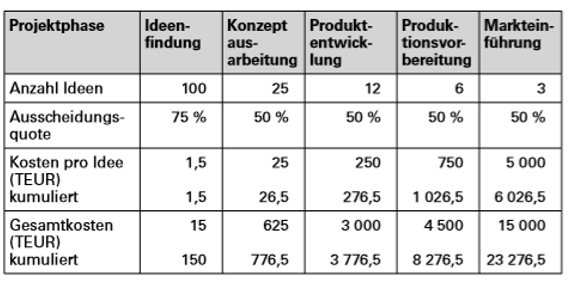
\includegraphics{ideenfilterung.png}
	\caption{Ausscheidungsquoten und Kostenentwicklung}
	\label{img:filterKosten}
\end{figure}

\subsection{Ideenbewertung}
Der Kern einer Ideenbewertung sind die Kriterien, anhand derer über eine Idee geurteilt wird.
Aus diesem Grund ist es wichtig, die Kriterien sorgfältig zu definieren. Werden die Kriterien falsch oder nicht sorgfältig gewählt,
so kann dies zu Ablehnungs- oder Annahmefehlern führen. 
Ablehnungsfehler bezeichnen Ideen, die fälschlicherweise abgelehnt wurden, obwohl sie bei genauerer Betrachtung 
zielführend gewesen wären. Das Gegenteil sind Annahmefehler, hier wird eine Idee weiterverfolgt, obwohl diese nicht zum Ziel führt. 
Während Ablehnungsfehler zu einer Verzögerung in der Entwicklung führen können, hinterlassen Annahmefehler verschwendete Zeit und verschwedetes Geld.\\

Kriterien lassen sich grundsätzlich in zwei Kategorien unterteilen. Allgemeine Kriterien und Aufgabenspezifische Kriterien.
\textbf{Allgemeine Kriterien} lassen sich auf verschiedene Ideen und Anwendungsfälle übertragen.
Um allgemeine Kriterien zu definieren, ist es nicht notwendig, die konkrete Aufgabe zu kennen. 
Die häufigsten allgemeinen Kriterien sind \textit{Attraktivität}, \textit{Realisierbarkeit} und 
\textit{Disruptionspotential}. Es ist erkennbar, dass es sich hierbei um grundsätzliche Kriterien handelt, die unabhängig von einer Thematik sind.\\
\textbf{Aufgabenspezifische Kriterien} hingegen erfordern genaue Kenntnisse der Aufgabenstellung. Es muss klar sein, welches 
konkrete Kundenbedürfnis mit einer Idee befriedigt werden soll. Auch verschiedene Markttrends müssen hierbei beachtet werden. 
Diese haben oft entscheidenen Einfluss auf die Erfolgschancen. Aufgabenspezifische Kriterien müssen für jede Aufgabe beziehungsweise jedes Ziel 
individuell formuliert werden.

\subsection{Kriterien der Ideenbewertung nach Zephram}
Auch Zephram teilt die Kriterien in zwei Kategorien ein. Allerdings setzt Zephram einen anderen Fokus und verfolgt 
damit ein anderes Ziel.\\

\textbf{Randbedingungen} beschreiben die Eigenschaften, die eine Idee haben muss
beziehungsweise nicht haben darf. Sie sind absolut und werden oft als \textit{Muss-Kriterien}
und \textit{Darf-Nicht-Kriterien} bezeichnet.
Typische Randbedingungen sind beispielsweise die \textit{Kosten}. 
Es wird festgelegt welchen Betrag eine Ideenumsetzung maximal kosten darf. 
Weitere typische Randbedingungen sind \textit{Fit}, die Idee muss zum Unternehmensimage passen, oder \textit{Ressourcen}, die Ressourcen für die
Umsetzung müssen vorhanden sein. 
Randbedingungen sind entweder erfüllt oder nicht. Je nachdem wird eine Idee verworfen oder weiterverfolgt. \\

\textbf{Erfolgskriterien} hingegen sind nicht absolut. Sie beschreiben Eigenschaften einer Idee, 
mit denen diese als erfolgreich gilt. Ziel ist es nicht, Ideen auszuschließen, sondern die
vielversprechendste Idee herauszufiltern. Das heißt im Umkehrschluss, alle anderen Ideen werden nicht 
verworfen, sondern zunächst nicht ausgewählt. Erfolgskriterien werden oft als \textit{Soll-Kriterien} bezeichnet. Um 
Erfolgskriterien einheitlich zu formulieren kann der Satz \textit{Je mehr..., desto besser"}.
Dieser Satz verdeutlicht, dass sich Erfolgskriterien nicht in \textit{erfüllt} und \textit{nicht erfüllt} aufteilen 
lassen. Typische Erfolgskriterien sind \textit{Gewinnpotential}, \textit{Wachstumspotential} oder \textit{Kundennutzen}.\\

\textbf{Kann-Kriterien} sollten bei der Bewertung von Ideen keine Rolle spielen. Es handelt sich hierbei 
um Kriterien, die nicht zwingend notwendig für den Erfolg einer Idee sind. Wird eine Idee anhand dieser Kriterien 
bewertet, so sind die Erfolgskriterien nicht gut gewählt und sollten demnach angepasst werden.\\

Beim \textbf{Formulieren} der Randbedingungen ist es wichtig, dass sich die Kriterien nicht
widersprechen. Folge wäre, dass alle Ideen aussortiert werden, da niemals alle Randbedingungen erfüllt sein können.
Als häufiges Beispiel ist hier die Forderung nach einer Systemausfallsicherheit von 98\% , aber dennoch eine 
kurzer Entwicklungszeit. 
Es kommt bei den Kriterien darauf an, das richtige Mittelmaß für die Aufgabe zu finden. 
Sowohl Randbedingungen wie auch Erfolgskriterien sollten zur Aufgabe passen. Eine weitere Schwierigkeit ist eine möglichst konkrete
Formulierung der Kriterien zu finden. \\

Beim \textbf{Anwenden} der Kriterien zur Bewertung von Ideen müssen zunächst die Randbedingungen angewandt werden. 
Dies sorgt bereits für eine starke Reduktion der Anzahl an Ideen. Um hierbei keine Fehler zu machen, wird 
ein Vier-Augen-Prinzip empfohlen. 
Schwieriger ist die anschließende Anwendung der Erfolgskriterien, da diese graduell sind, allerdings keine klar 
definierte Messskala besitzen. 
Es gibt einige Methoden, die die Arbeit mit Erfolgskriterien vereinfachen. Einige werden 
in der folgenden Liste aufgezählt: 
\begin{itemize}
    \item Punktekleben (Siehe in Kapitel \ref{sec:retro-punkte})
    \item Nutzwertanalyse
    \item Paarvergleichsmatrix
\end{itemize}
Die Methoden die von \ac{sac} angewendet werden, werden im Praxisteil genauer beschrieben. \cite{zephram:2018}

\subsection{Vorgehensweise nach Schawel-Billing}
Vorschlag von Schawel und Billing ist es, die Ideenbewertung in zwei Phasen zu unterteilen. Zunächst muss die gesamte Anzahl 
der Ideen verringert werden. Dies geschiet in der \textbf{Ideenkategorisierung}. Hierbei geht es darum, Ideen unter 
Oberbegriffen zusammenzufassen. Dies hilft vorallem dabei, ähnliche Ideen oder Überlappungen frühzeitig zu erkennen.
Zusätzlich hat diese Vorgehensweise den Vorteil, dass die gefundenen Kategorien später in Arbeitspakete überführt werden 
könnten. Anschließend können die Kategorien in der \textbf{Ideenbewertung} genauer Bewertet werden. 
Dies erfolgt anhand formulierter Kriterien. Für eine erste Einschätzung kann außerdem eine \ac{2d}-Matrix verwendet werden. 
Diese sollte die beiden Achsen \textit{Wirkung} und \textit{Realisierbarkeit} entgegenstellen. Ideen die eine geringe Wirkung haben und/oder 
schwer zu realisieren sind können so leicht identifiziert werden. \cite{schawel:2009}
\newpage
\section{SAP Analytics Cloud}\label{sec:sac}
Um die Kriterien zur Ideenbewertung bei \ac{sac} zu analysieren, ist es zunächst 
wichtig, ein Verständnis über den grundlegenden Aufbau und die Arbeitsweise sowie Hintergründe bezüglich 
existierender Kunden zu erhalten. 

\subsection{Produktbeschreibung}
\todo[inline]{Produktbeschreibung}

\subsection{Aufbau der Abteilung}
Die Abteilung die das Product \ac{sac} entwickelt, besteht aus weltweit verteilten Teams, 
die Verantwortung für verschiedene Bereiche des Produkts besitzen und diese Entwickeln. 
Die beiden Hauptstandorte sind Vancouver in Kanada und Walldorf in Deutschland. Weitere Teams sitzen beispielsweise in 
Shanghai oder Bangalore. Besonders bei globalen Entwicklungen ist es wichtig, Ideen bereits vorbewertet an andere Teams 
heranzutragen, denn der Kommunikationsaufwand zwischen mehreren Kontinenten ist kein zu unterschätzender Kostenfaktor. 
Die Struktur der Abteilung ist streng hierarchisch. Das bedeutet, dass viele Ideen bereits von Managern diskutiert und 
bewertet werden bevor sie bis zum Entwickler durchgereicht werden. Dennoch hat auch der Entwickler die Herausforderung, 
mehrere Ideen beziehungsweise Ideen zu bewerten und abzuwägen. Dabei handelt es sich meist, um detailierte Umsetzungsmöglichkeiten
einer Anforderung. 
Neben den Managern und Entwicklern besitzt die Abteilung außerdem Designer, die Oberflächen-Mockups entwickeln und auf
die \ac{ux} achten. Zuletzt aber besonders wichtig sind die Qualitätsverantwortlichen der Abteilung. Diese 
arbeiten mit den Entwicklern zusammen um durch Testkonzepte die Qualität des Produkts zu gewährleisten.

\subsection{Existierende Kunden}
Das Produkt war lange Zeit in der Entwicklung, wird seit einigen Jahren jedoch produktiv von Kunden verwendet. Besonders 
interessant im Bezug auf die Ideenbewertung sind einige wenige aber große Kunden, die sich durch Feedback in die 
Weiterentwicklung des Produkts einbringen. Diese Kunden melden zurück, welche Funktionen für sie sinnvoll oder 
zwingend notwendig sind. Sie haben so direkten Einfluss auf die Ideenbewertung. 

\subsection{Arbeitsweise in der Abteilung}
Die Abteilung arbeitet in einem individualisertem Scrum-Modus. Scrum ist eine agile Prozessmethode und basiert 
auf dem Grundsatz, dass es viele kleine Pakete einfacher zu entwickeln sind, als ein großes Paket. 
\begin{quote} Scrum basiert,[...], auf der Erkenntnis, daß es wesentlich einfacher ist, einen kleinen Bissen zu verdauen als einen großen.\cite{scrum:2018} \end{quote} 
Der Kern bei Scrum sind die vergleichsweise kurzen \textit{Sprints} nach denen ein Paket zum Kunden ausgeliefert wird. 
In \ac{sac} haben diese Sprints eine Länge von zwei Wochen. Dies bedeutet allerdings nicht, dass ein Paket 
innerhalb dieser Zeit fertiggestellt werden muss. Dies ist leider bei Funktionen, die von mehreren Teams an
verschiedenen Standorten, insbesondere mit unterschiedlicher Zeitzone entwickelt werden. Oft wird nach Fertigstellung eines 
Entwicklungspakets eine weiterer Sprint zum Stabilisieren und Testen angehängt, bevor die Funktionalität ausgeliefert wird.
Damit eine Funktionalität als bereit für die Auslieferung zum Kunden gilt, müssen Manager, Designer und Qualitätsverantwortlichen das 
Einverständnis geben. Dieses Konzept wird bei Scrum als \ac{dod} bezeichnet. 

\subsection{Team: Modeling}
Das Modeling-Team ist für einen Bereich der Anwendung verantwortlich, der viele Schnittpunkte zu anderen Teams besitzt.
\todo[inline]{Beschreibung der Funktionalität vom Modeling}

\todo[inline]{Beschreibung des Modelingteams}
Das Modeling besteht neben einem Manager aus zwei Architekten, die den Manager mit der Entscheidung über 
Entwicklungsaufgaben unterstützen und den gesamten Modeling-Bereich technisch überblicken. 
%!TEX root = ../seminararbeit.tex
\section{Retrospektive bei SAP Analytics Cloud}\label{sec:retro}
\subsection{Retrospektive}
Im Team \textit{Modeling} werden in regelmäßigen Abständen Retrospektiven durchgeführt. 
Die Retrospektiven sind ein Konzept von Scrum. Sie haben das Ziel den vergangen Sprint zu anlysieren und aus den Fehlern zu lernen, aber auch  auf positive 
Geschehnisse hinzuweisen um so das Team in Effizienz, Zusammenarbeit und Geimschaftsgefühl zu verbessern. \cite{retro:2018}. Ziel ist es die \\
Die Retrospektiven im \textit{Modeling} finden nicht nach jedem Sprint statt, sondern alle 6 Wochen.
\autoref{img:retroAblauf} zeigt einen häufigen Ablauf einer Retrospektive. Je nach aktuellen Situationen können die 
verwendeten Methoden angepasst werden. Im Bezug auf die Thematik dieser Arbeit, Kriterien zur Ideenbewertung,  
sind besonders die Punkte \textit{Gewichtung der gefundenen Probleme} und \textit{Lösungsideen bewerten} relevant.
\begin{figure}[ht]
	\centering
	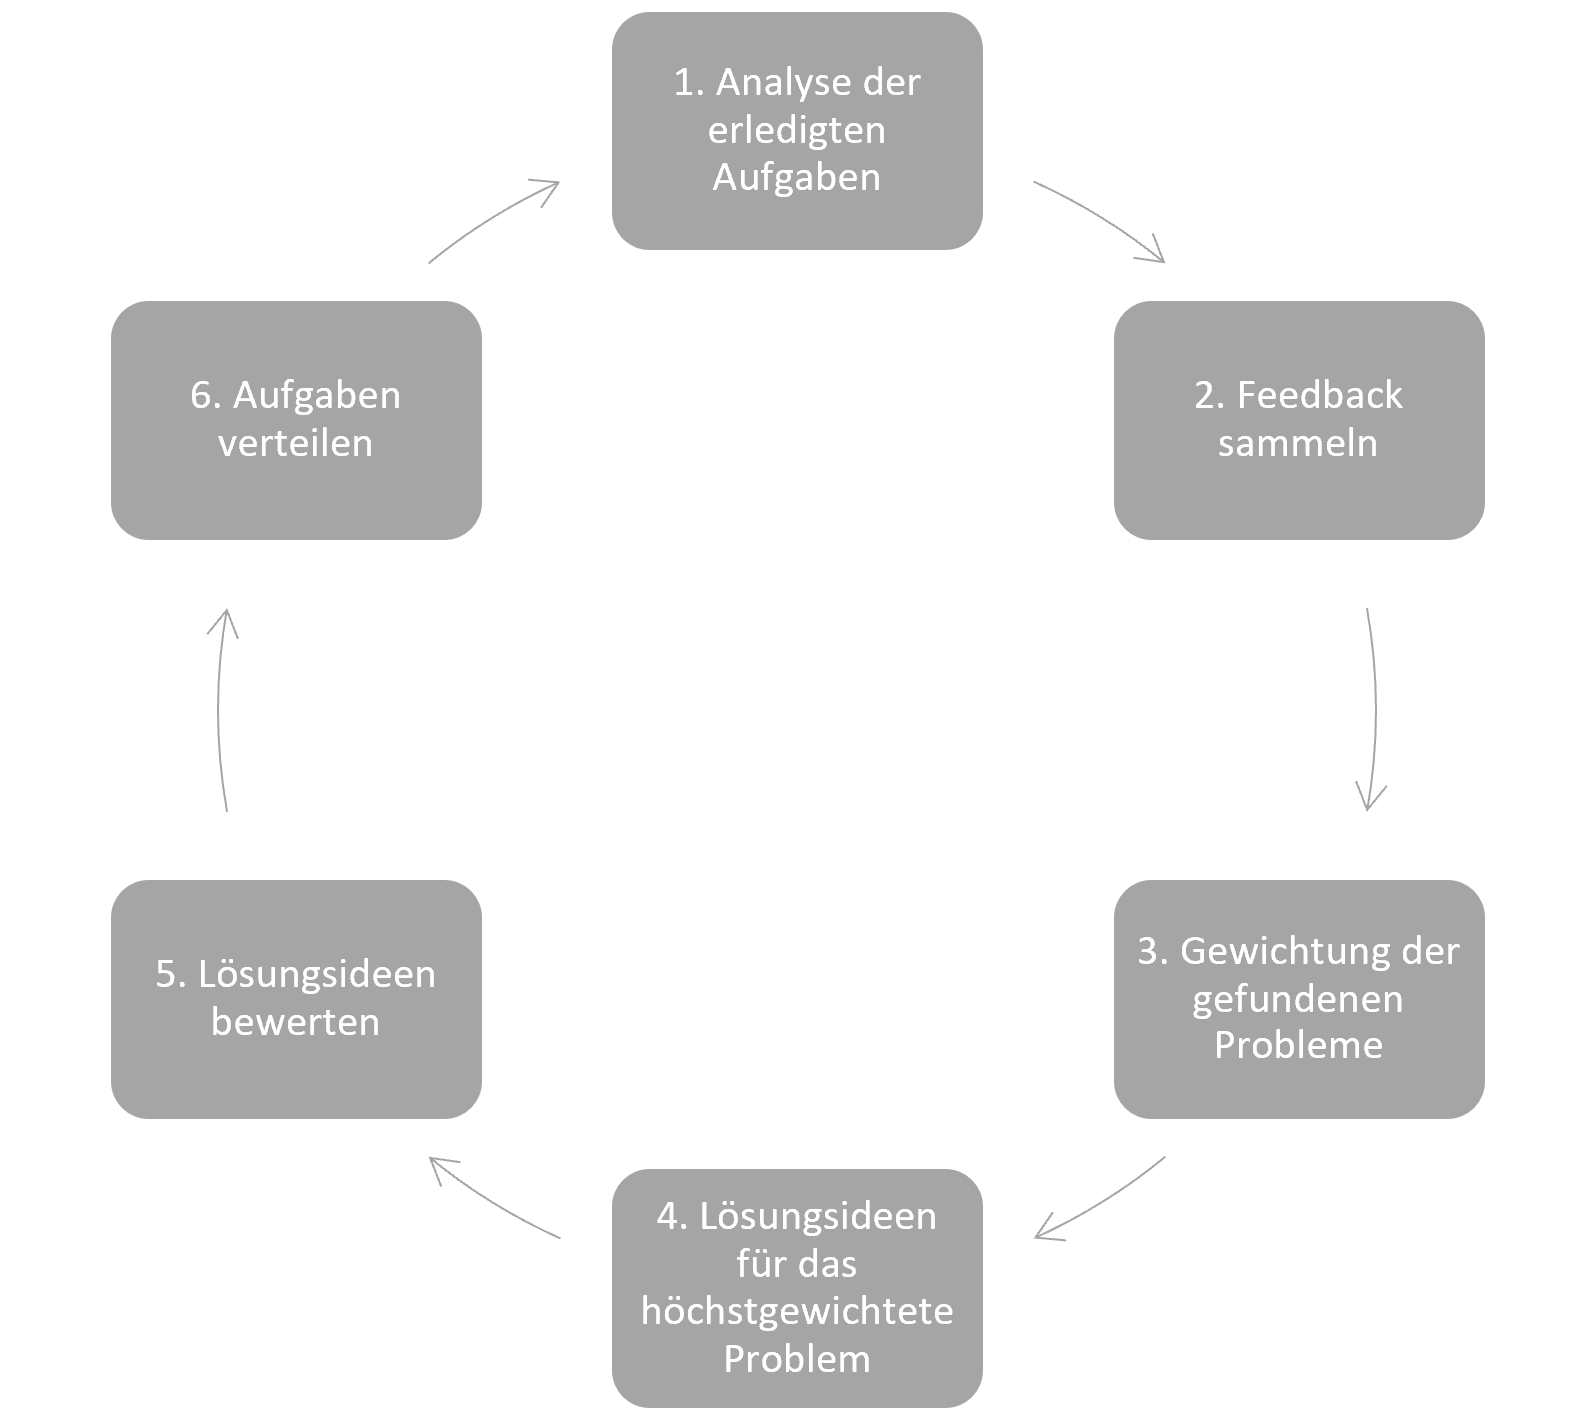
\includegraphics[width=10cm]{retroAblauf.png}
    \caption{Ablauf einer Retrospektive im Modeling}
	\label{img:retroAblauf}
\end{figure}
\begin{enumerate}
    \item In einer Retrospektive wird zunächst auf die letzte Restrospektive zurück geblickt. Es wird überprüft ob die Ideen der letzen 
        Retrospektive umgesetzt wurden.
    \item Anschließend geht es darum neue Ideen für die nächsten 6 Wochen zu sammeln. Jedes Team-Mitglied
        hat die Möglichkeit positive und negative Geschehnisse vorzustellen. 
    \item Die negativen Geschehnisse werden in Kategorien zusammengefasst. 
    \item Als nächstes werden die negativen Geschehnisse bewertet. Ziel ist es, das schwerwiegendste Problem zu finden beziehungsweise 
    das Problem, dass die meisten verbessern möchten. Jedes Team-Mitglied kann hierzu eine Bewertung abgeben. 
    \item Für das ausgewählte Problem müssen nun Lösungen gefunden werden. Jedes Teammitglied kann Ideen beisteuern. 
    \item Nun müssen die Ideen bewertet werden und konkrete Aufgaben an Team-Mitglieder verteilt werden.
\end{enumerate}

\subsection{Bewertung der Probleme}\label{sec:retro-punkte}
Für die Abstimmung darüber, welches der Probleme angegangen wird, zeigte sich die Methode \textit{Priorisierung mit Punkten} 
als geeignet. 
\begin{quote}
    Die Grundidee ist die, dass jeder Teilnehmer eine gewisse Zahl an Stimmen (z.B. in Form von Klebepunkten [...]) bekommt, die er auf die generierten Ideen verteilen kann. \cite{dotmocracy:2011}
\end{quote} 
Dies ist eine schnelle Methode, die dennoch jeden einzelnen Teilnehner berücksicht. Ziel der Problembewertung ist es, das Problem zu 
finden, dass die meisten Team-Mitglieder beschäftigt. Das bedeutet wiederum, dass hierbei nicht nach vorgegebenen Kriterien 
vorgegangen wird, sondern dass, die indivuellen und subjektiven Meinungen der Team-Mitglieder gruppiert werden sollen. 
Kriterium der Ideenbewertung ist ausschließlich, die eigene Meinung wiederzugeben. Dies wird explizit erwähnt, 
da eine Gefahr dieser Methode beispielsweise der Herdentrieb sein kann. Das bedeutet, dass ein Team-Mitglied 
ein Problem wählt, da es bereits die meisten Punkte besitzt. So könnte es zu Ablehnungs- bzw. Annahmefehler des Problems kommen. \cite{derby:2012}
Ein weiteres implizites Kriterium ist, dass das Problem lösbar sein sollte. Dies ist zwar eigentlich ein Teil der Ideenbewertung, 
dennoch wird ein Problem, das nicht gelöst werden kann, von den meisten Mitgliedern nicht gewählt. 

\subsection{Bewertungskriterien für Ideen}\label{sec:retro-kriterien}
Im Gegensatz zur Bewertung der Probleme, gibt es bei der Auswahl der Lösungen einige Randbedingungen
und Erfolgskriterien die beachtet werden müssen.

\textbf{Randbedingungen}
\begin{enumerate}
    \item Die Lösungsidee, muss von Team-Mitgliedern umsetzbar sein. Das beudeutet es sollten keine Ideen gewählt werden, die ausschließlich von Mitarbeitern auserhalb des Teams
    umgesetzt werden können. Zum Beispiel kann das Problem, dass es keine Klimaanlage in den Büros gibt, lediglich an die zuständige Stelle weitergeleitet werden.
    Keine Team-Mitglied kann die Idee, eine Klimaanlage einzubauen umsetzen. 
    \item Eine weitere Randbedingung ist, dass die Ideen innerhalb der folgenden 6 Wochen umgesetzt werden können muss. Zu Beginn der 
    nächsten Retrospektive wird das Ergebnis analysiert.
    \item Besonders wichtig ist, dass die Idee zur Lösung des Problems beiträgt. Oftmals ist es nicht möglich ein Problem vollständig zu lösen. 
    Deshalb sind Kompromisse möglich. Das Teammitglied, welches das Problem angesprochen hat, sollte diese Randbedingung bewerten. So kann 
    wird abgesichert, dass auch alle das Problem richtig verstanden haben und so eine sinnvolle Lösung gewählt werden kann. 
\end{enumerate}
\textbf{Erfolgskriterien}
\begin{enumerate}
    \item "Je schneller die Idee, zur Lösung des Problems führt, desto besser." 
    \item "Je effektiver die Idee, zur Lösung des Problems führt, desto besser."
    \item "Je mehr Mitarbeiter von der Lösung profitieren, desto besser."
\end{enumerate}

Das bedeutet zum einen, eine Abwähgung zwischen Aufand und Nutzen der Lösung und zum anderen sollten möglichst viele Mitarbeiter 
von Lösung profitieren. Deshalb wird die Entscheidung über die Umsetzung eine Idee, im gesamten Team besprochen. Zusätzlich ist es wichtig,
dass die Lösung. 
\section{Einführung neuer Features bei SAP Analytics Cloud}\label{sec:kaptiel}

\subsection{Einführung neuer Features}
\begin{itemize}
    \item Managemententscheidungen
    \item Kundenanforderungen/wünsche
    \item Welche Features werden umgesetzt?
    \item Umsetzung: Zusammenarbeit verschiedener Teams, Verantwortlichkeit
    \item Umsetzbarkeit von Features
    \item Architekturkonzept
    \item Entwickler in Zusammenarbeit mit Designern
\end{itemize}
\section{Fazit}\label{sec:fazit}


%\printacronyms{}
\printbibliography{}
\end{document} 